\chapter{Análise Teórica}

A compreensão prévia do circuito por meio da teoria de grandes e pequenos sinais é a base metodológica que permite prever o comportamento do amplificador emissor comum e diagnosticar eventuais discrepâncias na bancada. Nesta seção, modela-se o circuito dinâmico como um quadripolo após a determinação rigorosa do seu ponto de operação quiescente.

\begin{figure}[htbp]
	\centering
	
\includegraphics[width=0.7\textwidth]{FIGURAS/esquematico_circuito.png}
	\caption{Esquemático do amplificador emissor comum com realimentação.}
	\label{fig:esquematico}
\end{figure}

\section{Análise Algébrica: Modelagem de Grandes e Pequenos Sinais}

Pelo princípio da superposição, a componente DC do circuito é isolada assumindo que os capacitores de acoplamento ($C_{C1}$ e $C_{C2}$) e o capacitor de desvio do emissor ($C_E$) apresentam impedância infinita (circuitos abertos) para frequência nula. As fontes de excitação AC são inativadas (curto-circuitadas).

O TBJ é então substituído pelo seu modelo equivalente de grandes sinais, onde a junção base-emissor é aproximada por uma fonte de tensão constante $V_{BE0}$ e o coletor é modelado por uma fonte de corrente dependente, ditada pela relação do ganho de corrente contínua $I_C = \beta I_B$.

\begin{figure}[htbp]
	\centering
	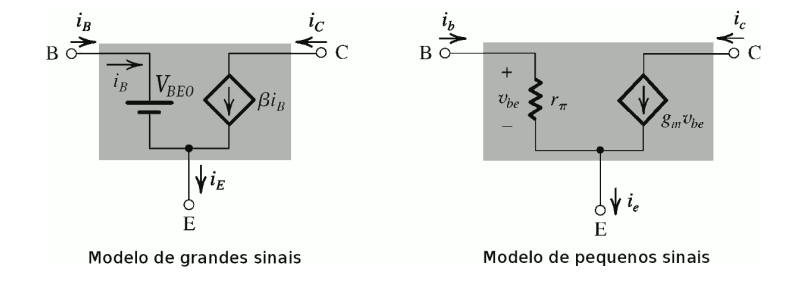
\includegraphics[width=0.8\textwidth]{FIGURAS/modelos_grandes_e_pequenos_sinais.png}
	\caption{Modelos equivalentes do TBJ: Grandes Sinais (DC) à esquerda e Pequenos Sinais (AC) à direita.}
	\label{fig:modelos}
\end{figure}

Aplicando a Lei de Kirchhoff das Tensões (LKT) na malha externa que engloba a fonte de alimentação, o resistor de coletor, o resistor de realimentação, a junção base-emissor e o resistor de emissor, equaciona-se:
\begin{equation}
	V_{CC} - R_C(I_C + I_B) - R_f I_B - V_{BE0} - R_E I_E = 0
\end{equation}

Substituindo as relações ativas $I_C = \beta I_B$ e a lei dos nós $I_E = (\beta + 1)I_B$, a expressão analítica exata para a corrente de base ($I_B$) resulta em:
\begin{equation}
	I_B = \frac{V_{CC} - V_{BE0}}{R_f + (\beta + 1)(R_C + R_E)}
\end{equation}

A partir de $I_B$, definem-se as tensões nodais do ponto de operação ($Q$):
\begin{itemize}
	\item $V_E = R_E (\beta + 1)I_B$
	\item $V_B = V_E + V_{BE0}$
	\item $V_C = V_{CC} - R_C(\beta + 1)I_B$
\end{itemize}

Para a resposta AC, o circuito é tratado sob a ótica de pequenos sinais. Os capacitores tornam-se curtos-circuitos e a fonte $V_{CC}$ é aterrada. O transistor assume o modelo $\pi$-híbrido (Figura \ref{fig:modelos}, à direita). Tratando a topologia como um quadripolo cujas portas de entrada e saída são delimitadas pelos nós $a$ e $b$ (ver Figura \ref{fig:esquematico}), extraem-se os parâmetros $g$ a partir das análises nodais:
\begin{align}
	g_{22} &= \left. \frac{I_2}{V_2} \right|_{I_1=0} = R_C \parallel R_f \label{eq:g22} \\
	g_{21} &= \left. \frac{V_2}{V_1} \right|_{I_2=0} = \left( \frac{1}{R_f} - g_m \right) g_{22} \\
	g_{12} &= \left. \frac{I_1}{I_2} \right|_{V_1=0} = - \frac{g_{22}}{R_f} \\
	g_{11} &= \left. \frac{V_1}{I_1} \right|_{V_2=0} = \frac{1}{r_\pi} + \frac{1}{R_f}(1 - g_{21})
\end{align}

\section{Estudo de Caso Analítico (Valores Nominais)}

Alimentando as equações com os valores estipulados no roteiro ($V_{CC} = 12\text{ V}$, $R_C = 4,7\text{ k}\Omega$, $R_E = 470\text{ }\Omega$, $R_f = 150\text{ k}\Omega$, $\beta = 150$, $V_{BE0} = 0,7\text{ V}$), determina-se algebricamente o ponto quiescente:
\begin{itemize}
	\item $I_B \approx 12,14\ \mu\text{A}$
	\item $I_C \approx 1,821\text{ mA} \quad \text{e} \quad I_E \approx 1,833\text{ mA}$
	\item $V_E \approx 0,861\text{ V} \quad , \quad V_B \approx 1,561\text{ V} \quad \text{e} \quad V_C \approx 3,385\text{ V}$
\end{itemize}

A verificação do modo ativo confirma-se, uma vez que a junção base-emissor está diretamente polarizada ($v_{BE} = 0,7\text{ V}$) e a junção base-coletor reversamente polarizada ($v_{CB} = 1,824\text{ V} > -0,4\text{ V}$). Com a polarização estável, os parâmetros diferenciais valem $g_m \approx 54,6\text{ mA/V}$ e $r_\pi \approx 2,75\text{ k}\Omega$. Resolvendo as equações do quadripolo:
\begin{itemize}
	\item $g_{11} \approx 2,03\text{ mS}$ \quad ; \quad $g_{12} \approx -0,0304$
	\item $g_{21} \approx -248,8\text{ V/V}$ \quad ; \quad $g_{22} \approx 4,56\text{ k}\Omega$
\end{itemize}

Ao acoplar uma carga $R_L$ na porta 2, o modelo prevê que uma entrada $V_1 = 30\text{ mV}$ produziria $V_2 \approx 0,97\text{ V}$ para $R_L = 680\ \Omega$, e expressivos $V_2 \approx 6,84\text{ V}$ para $R_L = 50680\ \Omega$, evidenciando a natureza de um forte estágio de ganho de tensão dependente da carga.

\section{Análise Investigativa Complementar: O Impacto Reversivo do Ganho $\beta$}

Durante as aferições de bancada, o amplificador apresentou um comportamento anômalo severo: o ganho previsto não ocorreu, com a saída não ultrapassando a faixa dos dezenas de milivolts ($V_2 < 30\text{ mV}$), configurando uma falha operacional. Para diagnosticar este fenômeno, propõe-se uma análise física focada nas reais características do componente utilizado.

\begin{figure}[htbp]
	\centering
	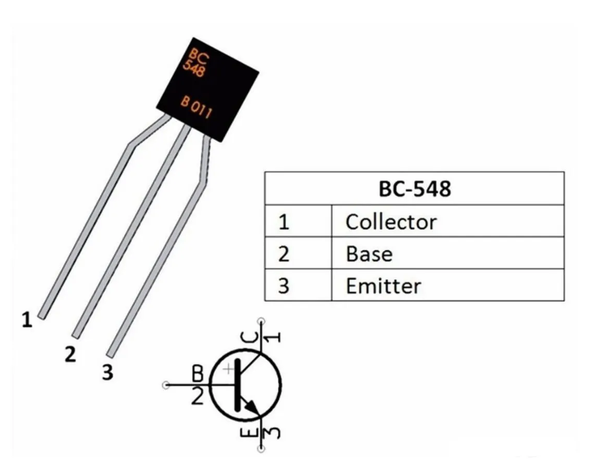
\includegraphics[width=0.4\textwidth]{FIGURAS/bc548_foto.png}
	\caption{Encapsulamento e disposição dos terminais do transistor BC548 empregado na bancada.}
	\label{fig:bc548}
\end{figure}

O transistor utilizado foi um BC548 (Figura \ref{fig:bc548}). Ao contrário do $\beta = 150$ nominal sugerido, transistores desta família (especialmente os sufixos B e C) frequentemente apresentam ganho de corrente contínua na faixa de $\beta \approx 350$. 

A topologia de polarização com $R_f = 150\text{ k}\Omega$ é extremamente dependente do parâmetro $\beta$. Refazendo os cálculos do ponto de operação com o ganho real do componente ($\beta = 350$):
\begin{equation}
	I_B = \frac{11,3}{150\text{k} + 351(5,17\text{k})} \approx 5,75\ \mu\text{A} \implies I_C = 350 \cdot 5,75\ \mu\text{A} \approx 2,01\text{ mA}
\end{equation}

Esta corrente de coletor impõe uma queda de tensão drástica sobre $R_C$:
\begin{equation}
	V_C = 12 - 4700(2,01\text{m}) \approx 2,53\text{ V}
\end{equation}
Com $V_E \approx 0,94\text{ V}$ e $V_B \approx 1,64\text{ V}$, a tensão coletor-base cai para $v_{CB} \approx 0,89\text{ V}$. Embora numericamente ainda no modo ativo, esta estreita margem deixa o circuito extremamente suscetível a variações térmicas de $V_{BE0}$. Qualquer aumento de temperatura diminui $V_{BE}$, aumentando a corrente de base e empurrando irreversivelmente o TBJ para a região de \textbf{saturação}. 

Na saturação, o modelo de pequenos sinais colapsa. O parâmetro da transcondutância ($g_m$) cai exponencialmente, e a junção base-coletor passa a atuar como um curto dinâmico. Isso justifica por completo o fato de o sinal de saída ter sido ceifado para níveis próximos ao sinal de entrada ($30\text{ mV}$).

Para resgatar a integridade do amplificador com um BC548 de $\beta = 350$, a teoria demonstra que a malha de realimentação deve ser atenuada. Aumentando-se $R_f$ para a faixa de $500\text{ k}\Omega$ a $1\text{ M}\Omega$:
\begin{equation}
	I_B = \frac{11,3}{500\text{k} + 351(5,17\text{k})} \approx 4,88\ \mu\text{A} \implies I_C \approx 1,70\text{ mA}
\end{equation}
Isso recuaria a tensão do coletor para um patamar seguro de $V_C \approx 3,97\text{ V}$, distanciando o TBJ da zona de saturação e restaurando a capacidade de excursão simétrica do sinal amplificado.